\documentclass{article}[a4paper, 11pt]
\usepackage[utf8]{inputenc}
\usepackage[swedish]{babel}
\usepackage{hyperref}
\usepackage{graphicx,float,tikz,pgfplotstable,pgfplots}

\begin{document}
	\title{\LaTeX första intrycket}
	\author{Mikael Leuf}
	\begin{titlepage}
		\maketitle
		\thispagestyle{empty}
	\end{titlepage}
	\pagebreak
	\begin{abstract}
		första intrycket av \LaTeX var att de såg ut och betedde sig som HyperText Markup Language(HTML).
	\end{abstract}
	\pagebreak
	\tableofcontents
	\thispagestyle{empty}
	\pagebreak

	\section{Runberg Snart hundra ordböcker}
		Ordböcker har blivit en stor genre i Projekt Runeberg. Redan i december 1998 digitaliserade vi "Biblisk ordbok" (1896) av Erik Nyström. 
		Vi hade då precis börjat införa faksimilutgåvor (med scannade bilder av boksidorna, inte bara text), och ville vi prova hur det fungerade för ordböcker. Det dröjde dock fem år till nästa försök, när sjätte upplagan av Svenska Akademiens ordlista (1889) digitaliserades i november 2003. Vid nyåret hade 70 år passerat efter Elof Hellquists bortgång och i mars 2004 digitaliserade vi hans "Svensk etymologisk ordbok" (1922), som fortfarande är en av våra mest besökta titlar. Åren 2004-2005 digitaliserades ytterligare fem ordböcker. 2007 tillkom det viktiga "Svenskt dialektlexikon" (1862-1867) av Johan Ernst Rietz. Men det var först 2009 som det tog fart. Sedan dess har vi digitaliserat flera ordböcker varje år. Sommaren 2011 började vi även digitalisera nyare ordböcker under antagandet att de egentligen inte är litterära verk i upphovsrättslagens mening, utan snarare kataloger (listor, förteckningar) med mycket kortare skyddstid. Hittills har ingen hört av sig med invändningar mot den tolkningen, som vi nu har använt i fyra år. Vårt senaste tillskott, en estnisk-tysk ordbok från 1970, är ett exempel på den tillämpningen. Sommaren 2011 satte vi också upp en temasida som samlar ordböckerna, hittills 98 titlar.

		För precis 20 år sedan satt vi och knappade in Bibeln. Den svenska översättningen från 1917 var fri från upphovsrätt. Redan 1991 hade delar av texten börjat spridas som datorfiler på nätet, men det gällde bara de stycken man helst läser, som bergspredikan, julevangeliet och skapelseberättelsen. För att få texten komplett måste ju även släktkrönikorna och annat läggas in. Det var ett stort arbete, som underlättas om fler hjälps åt. Men på den tiden fanns inga digitalkameror eller bredbandsanslutningar, mest långsamma modem. Tillräckligt många hade dock en Bibel, ett tangentbord och möjligheten att skicka e-post. En av oss gjorde en lista över Bibelns 66 böcker och 1189 kapitel. När en frivillig anmälde sig, blev hon eller han tilldelad ett kapitel att knappa in och sända in med e-post. När det fanns ett inskickat kapitel, gavs nästa frivilliga i uppdrag att korrekturläsa det. Tjugo frivilliga utförde dessa 2378 arbetsbeting inom loppet av två år. I mars 1996 var hela arbetet klart och finns sedan dess fritt och öppet tillgängligt för alla på vår sajt. \footnote{Texten är tagen direkt från \textit{\href{http://runeberg.org/}{Project Runeberg}}.}
	
		\subsection{Somalia}
			\begin{figure}[H]
				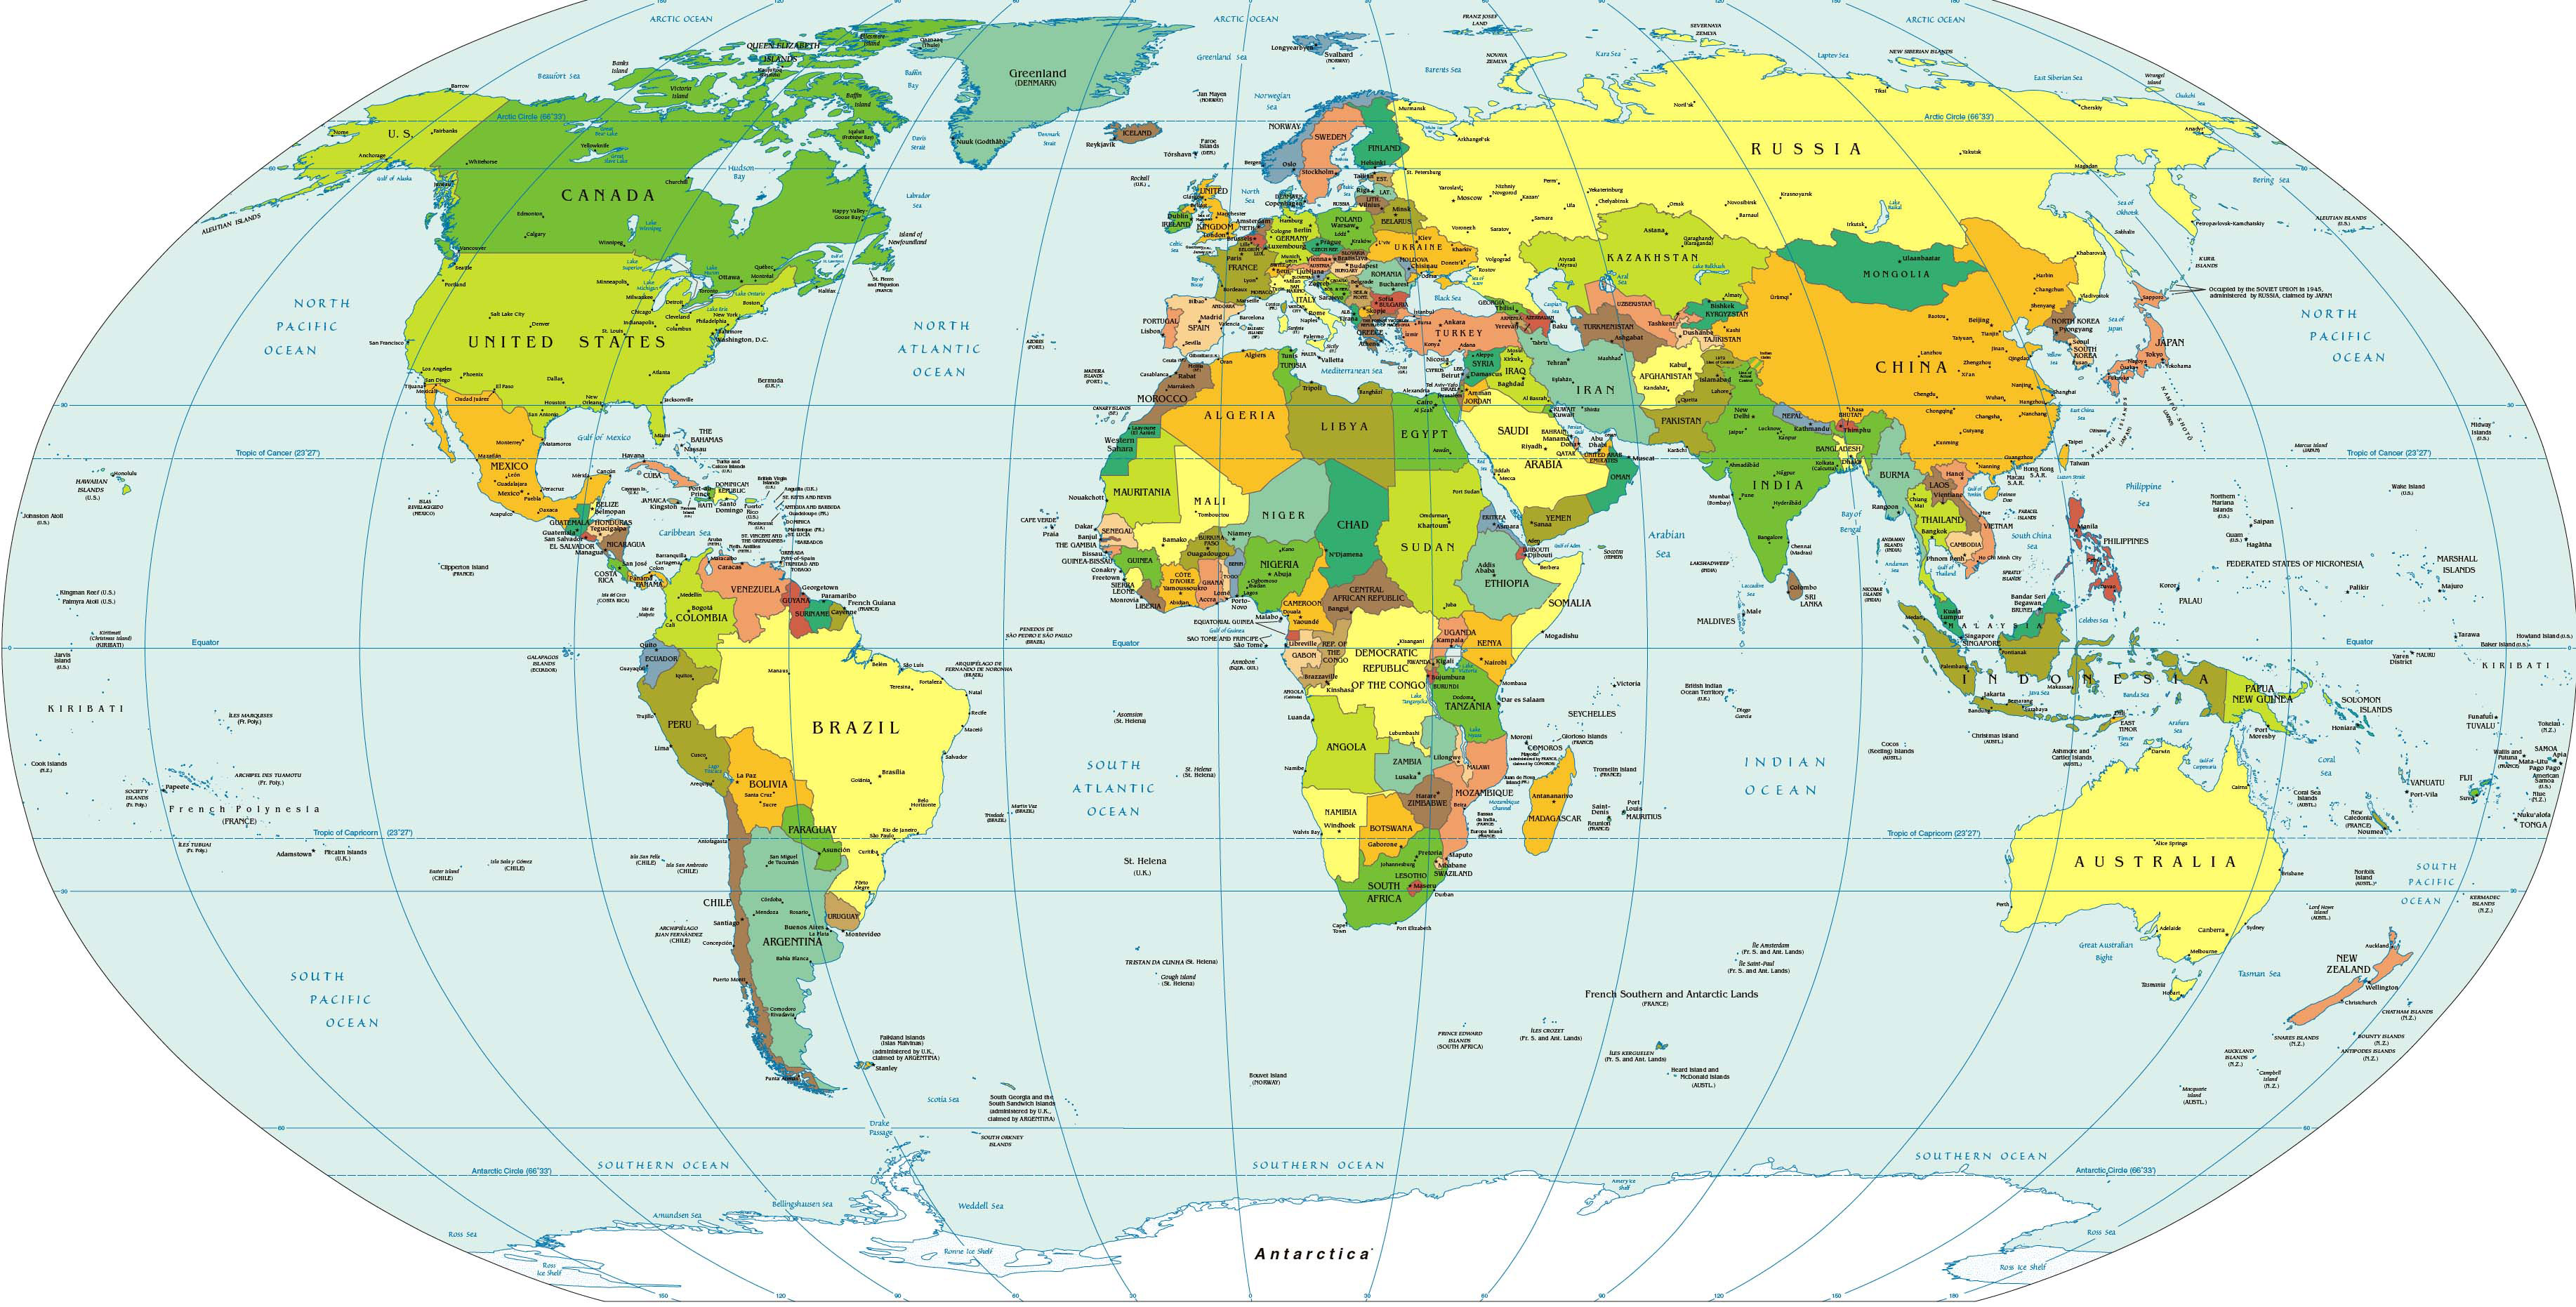
\includegraphics[viewport=2150 920 2270 1077, clip, angle=-12.34]{world}
				\caption{Somalia}
			\end{figure}

		\subsection{Diagram}
			\pgfplotstableread[row sep=\\,col sep=&]{
			parti    & X \\
			S		 &47.3	\\
			L		 &17.0	\\
			M		 &13.7	\\
			C		 &13.2	\\
			KD		 &1.8	\\
			V		 &5.2	\\
			MP		 &0		\\
			SD		 &0		\\
			ÖVR		 &0		\\
			}\mydata	
			\begin{figure}[H]
				\begin{tikzpicture}
					\begin{axis}[
						ybar,
						symbolic x coords={S,L,M,C,KD,V,MP,SD,ÖVR},
						ylabel={\large \%},
						xlabel={\large parti},
						]
						\addplot table[x=parti,y=X]{\mydata};
						\legend{Valresultat år 1964}
					\end{axis}
				\end{tikzpicture}
				\caption{Valresultat sveriger riksdag år 1964}
				\label{bar:chart}
			\end{figure}

			\subsubsection{Korsrefferens}
				Valresultat figur~\ref{bar:chart}

			\subsubsection{Tabell}
				%bind ihop alla 10 kolumner med en behändig liten konstruktion
				\begin{tabular}{|l*{10}{|c}}
					\hline
					År	&S	 	&L		&M		&C		&KD		&V	&MP&SD&ÖVR\\\hline
					1964&47,3	&17,0	&13,7	&13,2	&1,8	&5,2&0 &0 &0\\\hline
				\end{tabular}
\end{document}